\section{GPT-2 IOI: Recruitment and Mechanism}\label{sec:gpt2}

\subsection{Does attention increase imply recruitment?}\label{sec:gpt2-functional}

We apply FALI to GPT-2 Small on indirect object identification (IOI), perturbing the canonical primary Name Movers L9H6, L9H9, and L10H0 and using final-position IO-minus-subject logit difference as the task metric \citep{wang2023ioi}. The canonical confirmation cohort contains 15 low-level templates crossed with BABA/ABBA structure, 30 prompts per stratum, and four seeds, for 3600 prompts total. L10H2 and L10H10 are the primary candidate heads; L9H7 and L9H0 serve as same-layer architectural controls. Full sampling and bootstrap details are given in the Supplementary Information.

L10H2 satisfies the positive-recruitment criterion on the broad canonical cohort. Its conditional effect is $0.382$ (95\% CI $[0.341,0.424]$) and its conditional gain is $0.298$ ($[0.263,0.335]$). Its target attention also increases by $0.279$ ($[0.262,0.296]$).

L10H10 shows why attention adaptation is not sufficient evidence of recruitment. Its target attention increases even more, by $0.310$ ($[0.285,0.335]$), yet its conditional gain is negative, $-0.263$ ($[-0.302,-0.225]$), and its conditional effect is also negative, $-0.079$ ($[-0.111,-0.046]$). Figure~\ref{fig:gpt2-attention-recruitment}a therefore separates a visible attention response from the output-grounded functional response that FALI is designed to explain.

\begin{figure*}[t]
\centering
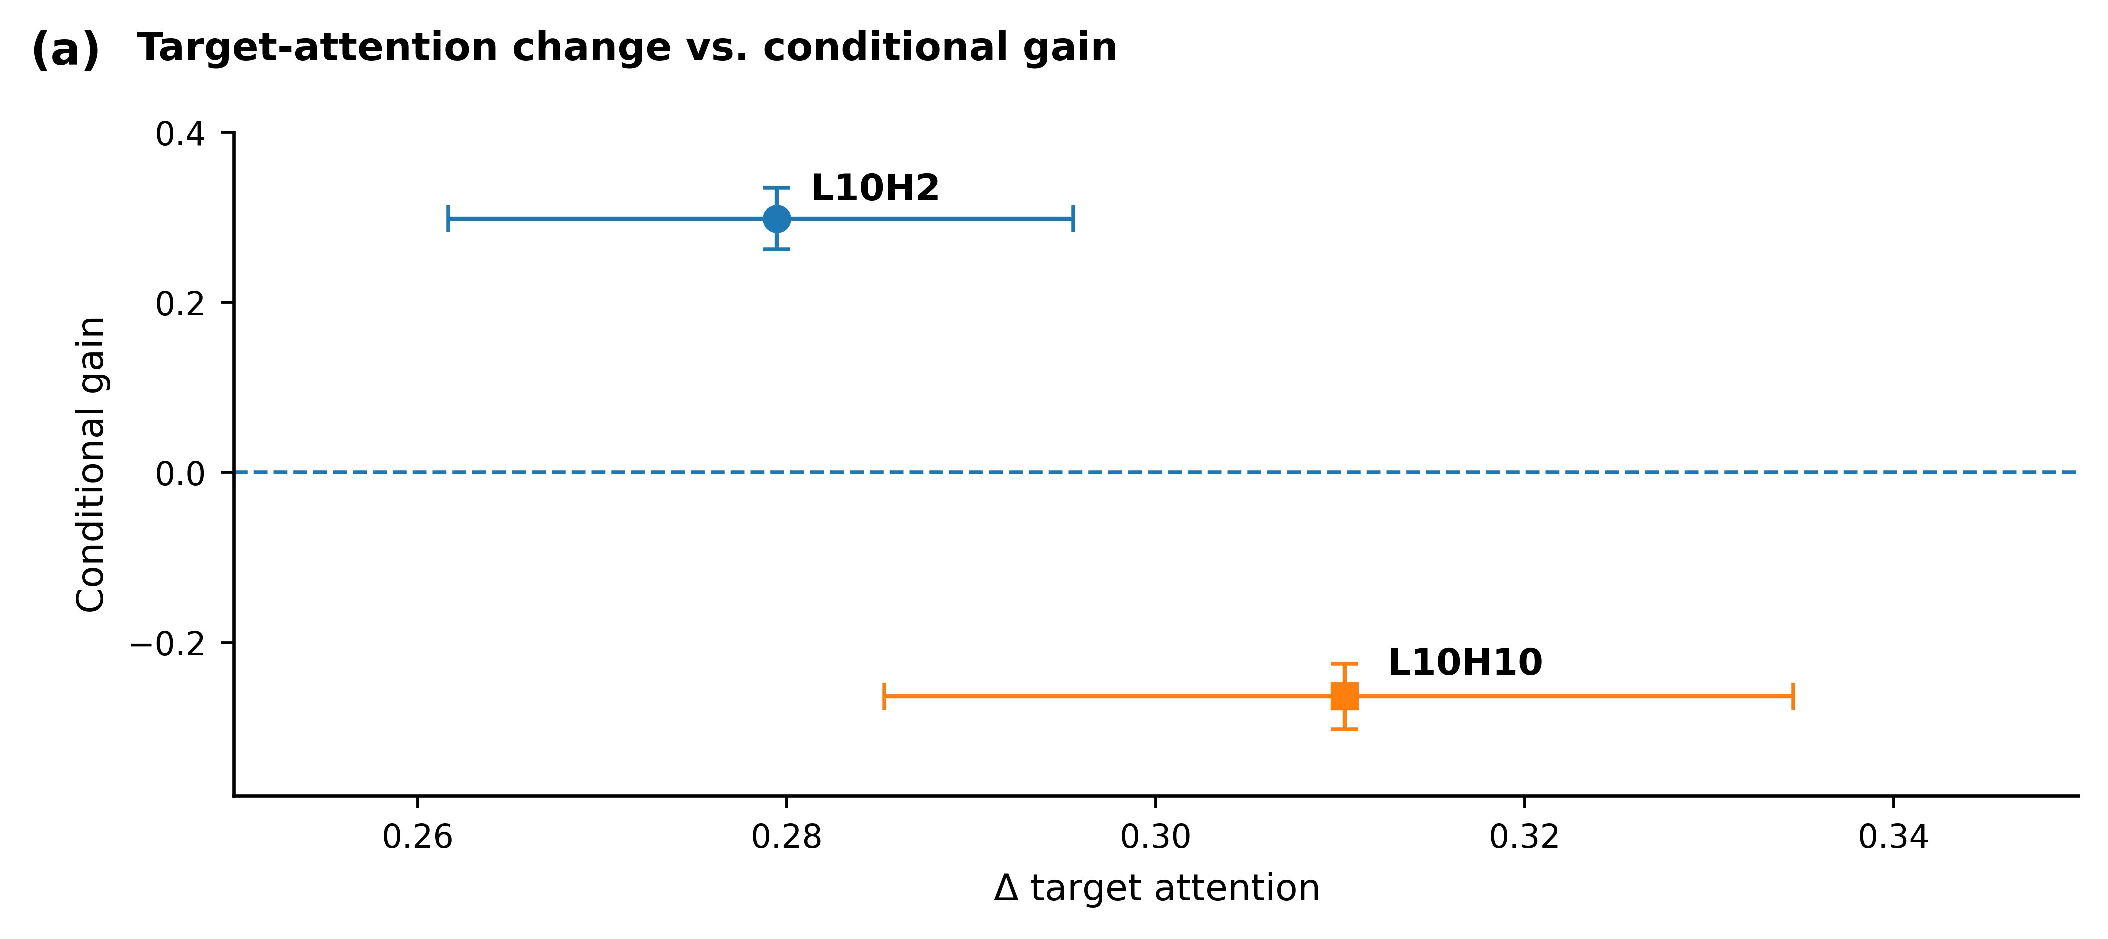
\includegraphics[width=0.95\textwidth]{figures/Fig4a.pdf}
\caption{\textbf{Target-attention adaptation is not sufficient for positive functional recruitment in GPT-2 IOI.}
(a) L10H2 and L10H10 both increase attention to the indirect-object target after ablation of the canonical primary Name Movers, but their conditional gains have opposite signs: L10H2 becomes more causally useful whereas L10H10 becomes less useful on the broad canonical distribution.
Points are exact balanced means; horizontal and vertical intervals are hierarchical 95\% bootstrap confidence intervals over the canonical template design.}
\label{fig:gpt2-attention-recruitment}
\end{figure*}


\subsection{What changes account for the GPT-2 response?}\label{sec:gpt2-fali}

For positively recruited L10H2, the coarse SCORE contribution is positive ($\Phi_{\mathrm{SCORE}}=0.445$), while value contributes approximately zero and surrounding context contributes negatively ($\phi_C=-0.146$). Within SCORE, the dominant pattern is target-positive and rival-negative: $\phi_T=0.783$ (95\% CI $[0.722,0.838]$) and $\phi_R=-0.341$ ($[-0.372,-0.311]$), with $\phi_O=0.0039$. The directional pattern holds in every seed and every canonical stratum, and remains when the legacy-overlapping template is excluded.

L10H10 exhibits the same fine-score signs despite its negative functional gain: $\phi_T=0.329$ ($[0.300,0.355]$) and $\phi_R=-0.126$ ($[-0.139,-0.113]$). Its positive SCORE contribution ($0.206$) is outweighed by a substantially negative surrounding-context contribution ($\phi_C=-0.471$). Figure~\ref{fig:gpt2-attention-recruitment}b--c shows both the fine score decomposition and the coarse score/value/context accounting.

This comparison is important for interpretation. A target-positive/rival-negative score reorganization is not synonymous with recruitment: it can occur in a head whose net causal usefulness decreases. Recruitment is defined by the output-grounded candidate effect; FALI then explains how the cross-state change is allocated under the intervention game. The same-layer controls L9H7 and L9H0 provide the complementary architectural case: their candidate score/value states do not change across the primary intervention, so their measured cross-state changes are assigned to surrounding context up to numerical precision.

\begin{figure*}[!t]
\centering
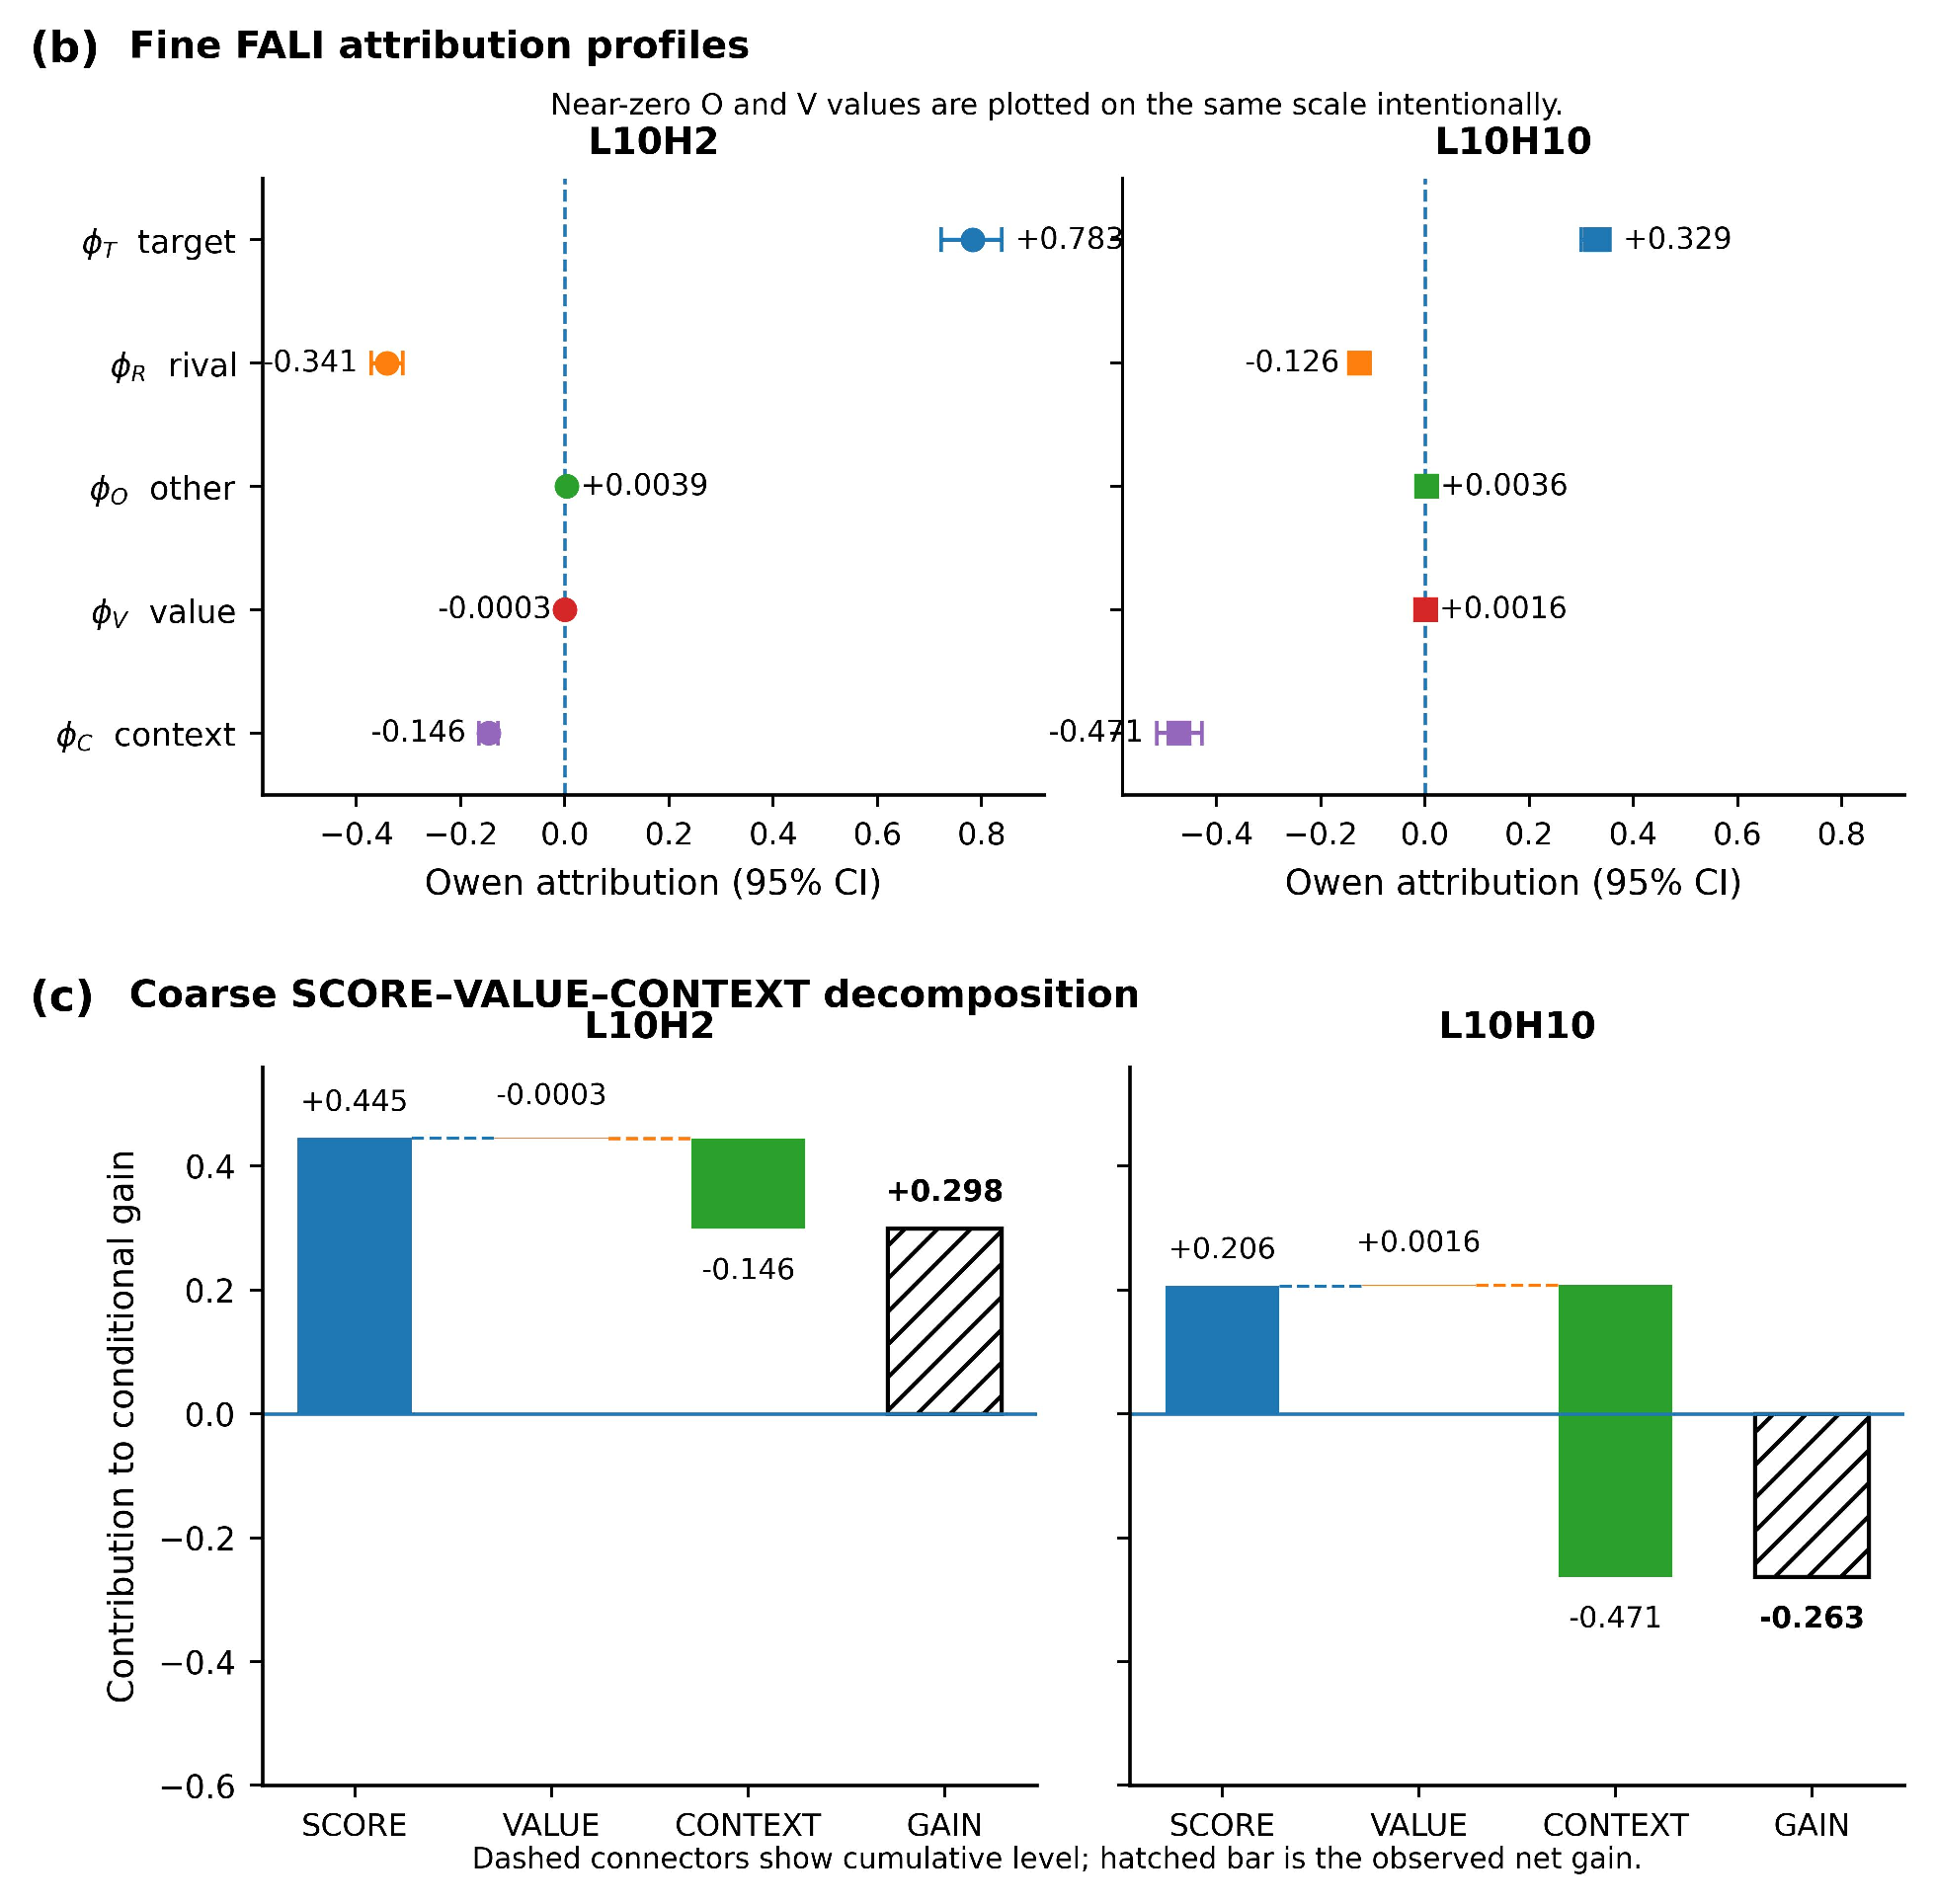
\includegraphics[width=0.92\textwidth]{figures/Fig4bc.pdf}
\par\smallskip
\noindent\textbf{Figure 4 (continued).} Fine and coarse FALI decomposition in GPT-2 IOI.
(b) Both L10H2 and L10H10 have positive target-score and negative rival-score contributions under the canonical FALI game; $O$ and $V$ remain near zero on the same plotted attribution scale.
(c) The coarse score/value/context decomposition explains why the same fine-score sign pattern does not imply the same functional response: L10H10 retains a positive SCORE contribution, but a substantially negative surrounding-context contribution outweighs it and produces a negative conditional gain.
Points are exact balanced means; intervals in panel (b) are hierarchical 95\% bootstrap confidence intervals. The context factor $C$ denotes surrounding-network/context contribution under the specified intervention game and is not a uniquely localized downstream mechanism.
\end{figure*}

